% (c) 2012 Claudio Carboncini - claudio.carboncini@gmail.com
% (c) 2012 Dimitrios Vrettos - d.vrettos@gmail.com
\chapter{Espressioni letterali e valori numerici}
\section{Lettere}
\subsection{Lettere per esprimere formule}
\begin{exrig}
 \begin{esempio}
 In tutte le villette a schiera di recente costruzione del nuovo quartiere Stella, vi è un
terreno rettangolare di larghezza~$12\unit{m}$ e lunghezza~$25\unit{m}$. Quanto misura la superficie del terreno?
\begin{center}
 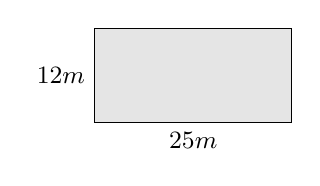
\begin{tikzpicture}[x=5mm, y=5mm,font=\small]
\definecolor{area}{gray}{0.9}
\draw [fill=area] (0,0) rectangle (5,2.4); 

\node[below] at (2.5,0) {$25\unit{m}$};
\node [left] at (0,1.2) {$12\unit{m}$};

\end{tikzpicture}
\end{center}

Il prodotto delle dimensioni rappresenta la misura richiesta:~$S=(25\cdot 12)\unit{m}^{2}=300\unit{m}^2$.
 \end{esempio}
\end{exrig}

Il semplice problema che abbiamo risolto è relativo ad un caso particolare; quel terreno con
quelle dimensioni. Ma se le dimensioni fossero diverse?

La procedura per determinare la misura della superficie ovviamente è sempre la stessa e la possiamo esprimere con la
formula~$A=b\cdot h$ nella quale abbiamo indicato con~$b$ la misura di una dimensione (base) e con~$h$ la misura dell'altra
dimensione (altezza), assegnate rispetto alla stessa unità di misura.

\osservazione La formula ha carattere generale e serve ogniqualvolta si chiede di determinare la superficie di un rettangolo,
note le misure delle dimensioni (base e altezza) rispetto alla stessa unità di misura.

In geometria si utilizzano tantissime formule che ci permettono di esprimere perimetro e
area delle figure piane, superficie laterale e totale e volume dei solidi. Nelle formule le lettere sostituiscono le
misure di determinate grandezze, tipiche di quella figura o di quel solido.

\ovalbox{\risolvi \ref{ese:8.1}}

\subsection{Lettere per descrivere schemi di calcolo}
\begin{exrig}
 \begin{esempio}
 L'insegnante chiede agli alunni di scrivere <<il doppio della somma di due numeri>>.

\begin{itemize*}
\item Antonella scrive:~$2\cdot (3+78)$;
\item Maria chiede <<Quali sono i numeri? Se non li conosco non posso soddisfare la richiesta>>;
\item Giulia scrive:~$2\cdot (a+b)$.
\end{itemize*}
Maria si è posta il problema ma non ha saputo generalizzare la richiesta. Antonella si è limitata ad un caso
particolare. Giulia ha espresso con una formula l'operazione richiesta dall'insegnante.
 \end{esempio}
\end{exrig}

\osservazione L'uso di lettere dell'alfabeto per indicare numeri ci permette di generalizzare uno schema di calcolo, cioè ci consente di scrivere un algoritmo.

\begin{definizione}
 Un'\emph{espressione letterale} o \emph{espressione algebrica} è uno schema di calcolo in cui compaiono numeri e lettere
legati dai simboli delle operazioni.
\end{definizione}

Per scrivere un'espressione letterale ci si deve attenere a regole precise, quelle stesse che utilizziamo per scrivere
espressioni numeriche.

Per esempio, la scrittura~``$3\cdot 4+$'' non è corretta, in quanto il simbolo~``$+$'' dell'addizione deve essere seguito da un
altro numero per completare l'operazione. Analogamente non è corretta l'espressione letterale~``$a\cdot c+$''.

Come nelle espressioni numeriche, anche nelle espressioni letterali le parentesi indicano la priorità di alcune operazioni rispetto ad altre.
La formula~$a\cdot (x+y)$ specifica ``il prodotto di un numero per la somma di altri due''. Essa è diversa da  $a\cdot x+y$
che rappresenta ``il prodotto di due numeri sommato a un terzo numero''.

\vspazio\ovalbox{\risolvii \ref{ese:8.2}, \ref{ese:8.3}, \ref{ese:8.4}}

\subsection{Lettere per esprimere proprietà}

Le proprietà delle operazioni tra numeri si esprimono con lettere per indicare che valgono per numeri
qualsiasi.
La scrittura ``$(a+b)+c=a+(b+c)$'', per esempio, esprime la proprietà associativa dell'addizione. In essa le lettere~$a$, $b$ e $c$ indicano
numeri qualsiasi. I due schemi di calcolo ci dicono che per sommare tre numeri è indifferente aggiungere alla somma
dei primi due il terzo oppure aggiungere al primo la somma degli altri due.

\vspazio\ovalbox{\risolvii \ref{ese:8.5}, \ref{ese:8.6}, \ref{ese:8.7}, \ref{ese:8.8}, \ref{ese:8.9}, \ref{ese:8.10}, \ref{ese:8.11}, \ref{ese:8.12}}

\section{Il valore numerico di un'espressione letterale}

Ogni espressione letterale rappresenta uno schema di calcolo in cui le lettere che vi compaiono sostituiscono numeri.
L'espressione letterale

\[2\cdot x^{2}+x\]

\noindent traduce una catena di istruzioni che in linguaggio naturale sono così
descritte: ``prendi un numero ($x$); fanne il quadrato ($x^2$); raddoppia quanto ottenuto ($2\cdot x^2$); aggiungi al risultato il numero preso inizialmente ($2\cdot x^{2}+x$)''.

Questa catena di istruzioni si può anche rappresentare in modo schematico
\[x\quad\rightarrow\quad x^{2}\quad\rightarrow\quad~2\cdot x^{2}\quad\rightarrow\quad~2\cdot x^{2}+x\]
e può essere usata per istruire un esecutore a ``calcolare'' l'espressione letterale
quando al posto della lettera~$x$ si sostituisce un numero.

Calcoliamo il valore dell'espressione~$2\cdot x^{2}+x$, sostituendo alla lettera $x$ il numero naturale~5.
Seguiamo la schematizzazione~$x\rightarrow x^{2}\rightarrow~2\cdot x^{2}\rightarrow~2\cdot x^{2}+x$ e otteniamo:
$5\rightarrow~25\rightarrow~50\rightarrow~55$.
Il risultato è~$55$.
Più brevemente scriviamo~$5$ nell'espressione letterale al posto di~$x$: otteniamo l'espressione numerica~$2\cdot 5^{2}+5$
il cui risultato è~$55$.

E se al posto di~$x$ sostituiamo~$-5$? Otteniamo un risultato diverso? Eseguiamo la sostituzione di $x$ con $-5$ e abbiamo: $2\cdot (-5)^{2}+(-5)=\ldots$ Lasciamo a te il calcolo finale. Ti sarai accorto che il
risultato è cambiato.

 \begin{definizione}
In un'espressione letterale le \emph{lettere} rappresentano le \emph{variabili} che assumono specifiche quantità
quando vengono sostituite da numeri.
Chiamiamo \emph{valore} di un'espressione letterale il risultato numerico che si ottiene eseguendo le operazioni indicate dallo
schema di calcolo quando alle lettere sostituiamo un determinato numero. Il valore di un'espressione letterale dipende dal \emph{valore assegnato} alle sue variabili.
\end{definizione}

D'ora in poi quando scriveremo un'espressione letterale in cui compare
l'operazione di moltiplicazione, tralasceremo il puntino fin qui usato per evidenziare l'operazione.
Così l'espressione~$5\cdot a^{2}+\dfrac{3}{8}\cdot a\cdot b-7\cdot b^{2}$ verrà scritta in modo
più compatto~$5a^{2}+\dfrac{3}{8}ab-7b^{2}$.

\begin{exrig}
 \begin{esempio}
Calcolare il valore numerico della seguente espressione:~$3a(a-b)$ per~$a=1$, $b=1$.

\emph{Svolgimento}:~$3\cdot 1\cdot (1-1)=3\cdot 1\cdot 0=0$.
\end{esempio}
 \end{exrig}

\ovalbox{\risolvii \ref{ese:8.13}, \ref{ese:8.14}, \ref{ese:8.15}, \ref{ese:8.16}, \ref{ese:8.17}, \ref{ese:8.18}, \ref{ese:8.19}, \ref{ese:8.20}, \ref{ese:8.21}, \ref{ese:8.22}, \ref{ese:8.23},
\ref{ese:8.24}}

\section{Condizione di esistenza di un'espressione letterale}
Ti proponiamo adesso alcuni casi particolari per
l'espressione~$E=\dfrac{x-y}{3x}$.

\paragraph{Caso I}

\begin{center}
\begin{tabular*}{.2\textwidth}{@{\extracolsep{\fill}}*{3}{c}}
\toprule
$x$ & $y$ & $E$\\
1 & 1 & 0\\
\bottomrule
\end{tabular*}
\end{center}

Il numeratore della frazione è~0, mentre il denominatore vale~3; il
calcolo finale è dunque~$\frac{0}{3}=0$.
Vi sono, secondo te, altre coppie di valori $(x;y)$ che fanno
assumere ad~$E$ quello stesso valore?

\paragraph{Caso II}
\begin{center}
\begin{tabular*}{.2\textwidth}{@{\extracolsep{\fill}}*{3}{c}}
\toprule
$x$ &$y$ &$E$\\
0 &25 &?\\
\bottomrule
\end{tabular*}
\end{center}

Invece di mettere un valore ad~$E$, abbiamo messo punto di domanda
perché in questo caso il numeratore della frazione è~$-25$ mentre
il denominatore vale~0; il calcolo finale è dunque~$-{\frac{25}{0}}$, impossibile.
Vi sono, secondo te, altre coppie di valori $(x;y)$ che rendono
impossibile il calcolo del valore per~$E$?

Non possiamo allora concludere che per ogni coppia di numeri razionali~$(x;y)$ 
l'espressione~$E$ assume un numero razionale.
Per poter calcolare il valore di~$E$ non possiamo scegliere coppie aventi~$x$ 
uguale a zero.
Scriveremo quindi come premessa alla ricerca dei valori di~$E$ la \emph{Condizione di Esistenza} ($\CE$)~$x\neq~0$.

L'esempio appena svolto ci fa capire che di fronte a
un'espressione letterale dobbiamo riflettere sullo
schema di calcolo che essa rappresenta prima di assegnare valori alle
variabili che vi compaiono.

Se l'espressione letterale presenta una divisione in cui
il divisore contiene variabili, dobbiamo stabilire la~$\CE$, 
eliminando quei valori che rendono nullo il divisore.
Per comprendere la necessità di porre le condizioni
d'esistenza ricordiamo la definizione di divisione.

Quanto fa~15 diviso~5? In forma matematica:~$15:5=3$ perché $3\cdot 5=15$. Quindi, 
generalizzando~$a:b=c$ se~$c\cdot b=a$.

Vediamo ora cosa succede quando uno dei numeri è~0:

\begin{itemize*}
 \item quanto fa~$0:5$? Devo cercare un numero che moltiplicato per~5 mi dia~0: trovo solo~0; infatti~$0\cdot 5=0$.
 \item quanto fa~$15:0$? Devo cercare un numero che moltiplicato per~0 mi dia~15:
non lo trovo; infatti nessun numero moltiplicato per~0 fa~15. Quindi,
$15:0$ è impossibile perché non esiste alcun
$x$ per il quale~$x\cdot 0=15$.
 \item quanto fa~$0:0$? Devo cercare un numero che moltiplicato per~0 mi dia~0:
non ne trovo solo uno. Infatti, qualunque numero moltiplicato per~0
fa~0. Per esempio, $0:0=33$; infatti
$33\cdot 0=0$. Ma anche~$0:0=\np{-189,6}$;
infatti~$\np{-189,6}\cdot 0=0$. E anche $0:0=0$;
infatti~$0\cdot 0=0$. 
Ancora~$0:0=10^{99}$, infatti~$10^{99}\cdot 0=0$.
Quindi~$0:0$ è indeterminato perché
non è possibile determinare un unico~$x$ tale che~$x\cdot 0=0$,
ma per qualunque valore di~$x$ si ha~$x\cdot 0=0$.
\end{itemize*}

Consideriamo l'espressione letterale~$E=\dfrac{a-b}{a+b}$ dove~$a$ e~$b$ 
rappresentano numeri razionali.
Premettiamo:

\begin{enumeratea}
 \item la descrizione a parole dello schema di calcolo:
``divisione tra la differenza di due numeri e la loro
somma'';
 \item la domanda che riguarda il denominatore: ``quand'è che la somma di
due numeri razionali dà come rislutato~0?'';
 \item la~$\CE$: ``$a$ e~$b$ non devono essere numeri opposti''.
\end{enumeratea}

Siamo ora in grado di completare la tabella:
\begin{center}
\begin{tabular*}{.8\textwidth}{l@{\extracolsep{\fill}}*{5}{c}}
\toprule
$a$ & 3 &0 & $\frac{3}{4}$ &$-{\frac{5}{8}}$ & $-{\frac{19}{2}}$ \\
$b$ & $-3$ & $-{\frac{1}{2}}$ & 0 &$\frac{5}{8}$ & $-{\frac{19}{2}}$ \\
\midrule
$E=\frac{a-b}{a+b}$ & & & & &\\
\bottomrule
\end{tabular*}
\end{center}

Dalla~$\CE$, ci accorgiamo subito che la
prima coppia e la quarta sono formate da numeri opposti, pertanto non
possiamo calcolare il valore di~$E$ ad esse relativo. L'ultima
coppia è formata da numeri uguali pertanto la loro differenza è~0, così
il numeratore si annulla e quindi il valore di~$E$ è~0. 
Per la coppia~$\left(0;-\frac{1}{2}\right)$ il valore di~$E$ è~$-1$ mentre è~1 per
la coppia~$\left(\frac{3}{4};0\right)$.
La tabella verrà quindi così completata:

\begin{center}
\begin{tabular*}{.8\textwidth}{l@{\extracolsep{\fill}}*{5}{c}}
\toprule
$a$ & 3 &0 & $\frac{3}{4}$ &$-{\frac{5}{8}}$ & $-{\frac{19}{2}}$ \\
$b$ & $-3$ & $-{\frac{1}{2}}$ & 0 &$\frac{5}{8}$ & $-{\frac{19}{2}}$ \\
\midrule
$E=\frac{a-b}{a+b}$ &impossibile & $-1$& 1& impossibile&0\\
\bottomrule
\end{tabular*}
\end{center}

Cosa succede per la coppia~$(0;0)$?

\vspazio\ovalbox{\risolvii \ref{ese:8.25}, \ref{ese:8.26}, \ref{ese:8.27}, \ref{ese:8.28}, \ref{ese:8.29}, \ref{ese:8.30}, \ref{ese:8.31}, \ref{ese:8.32}}
\newpage

 % (c) 2012-2013 Claudio Carboncini - claudio.carboncini@gmail.com
% (c) 2012-2014 Dimitrios Vrettos - d.vrettos@gmail.com
\section{Esercizi}
\subsection{Esercizi dei singoli paragrafi}
\subsubsection*{\thechapter.1 - Funzioni}
%\begin{esercizio}
% \label{ese:\thechapter.1}
% Per le funzioni rappresentate nell'esempio~\ref{ex:D.1} a pagina~\pageref{ex:D.1}, completa:
%
% \begin{itemize*}
%\item figura~a:~$\Dom =\ID = \dotfill$; $\IM = \dotfill$; $f(a) = \dotfill$;
%\item figura~c:~$\Dom = \ID = \dotfill$; $\Cod = \IM = \dotfill; f(\dots)= 4$.
%\end{itemize*}
% \end{esercizio}

\begin{esercizio}
 \label{ese:\thechapter.1}
È vero che la corrispondenza che associa ad ogni regione italiana il suo capoluogo di provincia è una
funzione?

\begin{enumeratea}
\item Completa:~$\Dom = \ID = \dotfill$;
\item è vero che~$\IM = \{$città d'Italia$\}$?
\item completa~$f($Liguria$)=\dotfill$; $f(\dotfill)=$ Cagliari?
\end{enumeratea}
\end{esercizio}

\begin{esercizio}
 \label{ese:\thechapter.2}
Assegnati gli insiemi~$A=\{$mare, ruspa, fegato, generale$\}$ e~$B=\{$1, 2, 3, 4, 5, 6, 7, 8, 9$\}$ la corrispondenza
che associa ad ogni elemento di~$A$ il numero di lettere di cui è
composta la parola è una funzione?

\begin{enumeratea}
\item Rappresentala con grafico sagittale e stabilisci l'insieme immagine;
\item quale relazione sussiste tra~$B$ e~$\IM$?
\end{enumeratea}
\end{esercizio}

\begin{esercizio}
 \label{ese:\thechapter.3}
Quali tra le seguenti relazioni sono funzioni?
\begin{center}
 \begin{tabular}{*3{l}}
 \toprule
  Dominio & Codominio & Relazioni\\
\midrule
libri & autori & a ogni libro associa l'autore\\
canzoni & cantanti & a ogni canzone associa il cantante\\
portoni di una via & numeri & a ogni portone associa il numero civico\\
computer & sistemi operativi & a ogni computer associa il S.O. installato\\
canzoni & orari & a ogni canzone associa la sua durata\\
libri & numeri interi & a ogni libro associa il suo numero di pagine\\
studenti della classe & voti & a ogni studente associa il voto di matematica\\
materie & libri & a ogni materia associa i testi in adozione\\
\bottomrule
 \end{tabular}
\end{center}
\end{esercizio}

\begin{esercizio}
 \label{ese:\thechapter.4}
Si è ammessi a una facoltà universitaria se nel test
d'ingresso si è avuto un punteggio compreso tra~60
incluso e~100 incluso. La corrispondenza che associa ad ogni studente
che ha superato il test il punteggio ottenuto è una funzione? Se sì
di che tipo è la funzione?
\end{esercizio}


\begin{esercizio}
 \label{ese:\thechapter.5}
Spiega perché la funzione che associa a ciascuna
persona il suo codice fiscale è biunivoca.
\end{esercizio}

\subsubsection*{\thechapter.2 - Funzioni tra insiemi numerici}
\begin{esercizio}
 \label{ese:\thechapter.6}
Nella corrispondenza che associa ad ogni intero il suo valore assoluto (esempio~\ref{ex:8.5} a pagina~\pageref{ex:8.5}), è vero che scelto un qualunque numero naturale è
possibile determinare almeno un numero intero di cui è immagine?
Completate:~$f(\ldots\ldots) = 45.$
L'osservazione precedente permette di concludere che
tale funzione è suriettiva?
Fate la rappresentazione sagittale della funzione.
\end{esercizio}

%\pagebreak

\begin{esercizio}
 \label{ese:\thechapter.7}
Data la funzione~$y=x-2$ con dominio~$\insN-\{$0, 1$\}$ e codominio~$\insN$ completa l'analisi dell'esempio~\ref{ex:8.7} a pagina~\pageref{ex:8.7}:
\begin{enumeratea}
\item elementi diversi del dominio hanno immagini diverse, quindi tale funzione è iniettiva;
si ha anche~$\IM =\Cod= \insN$ e pertanto la funzione è suriettiva, quindi \dotfill;
\item preso~$y = 8$ sapresti trovare l'elemento del dominio di cui è immagine? \dotfill;
\end{enumeratea}
\end{esercizio}

\begin{esercizio}
 \label{ese:\thechapter.8}
Stabilisci se la funzione~$f:y=\dfrac{1}{x}$ è
iniettiva. Nell'insieme immagine c'è lo zero?

Completate~$\Cod = \IM =\ldots$
Completate la tabella
\begin{center}
\begin{tabular}{l*8{c}}
\toprule
$x\in \insQ_{0}$ & $-2$ & $-7/8$ & $+1$ & & & & $-1$ & \\
$y\in \insQ_{0}$ & & & & $+1/3$ & $-12/5$ & $-7/8$ & & $-1$\\
\bottomrule
\end{tabular}
\end{center}
\end{esercizio}

\begin{esercizio}
 \label{ese:\thechapter.9}
Consideriamo la funzione~$f$ che associa ad ogni numero razionale il suo triplo.

$\insQ\xrightarrow{f}\insQ$; la sua espressione in forma
analitica è~$f: y = \dots\dots\dots$

$\Dom = \ID = \insQ$; possiamo moltiplicare per~3 qualunque numero razionale.

$\Cod = \IM =\insQ$; infatti per ogni numero razionale $y$ c'è un numero razionale $x$ di cui $y$ è il triplo, basta dividere $y$ per 3.
%il triplo di un numero razionale è ancora un numero razionale.
%
%Rispondete:

\begin{enumeratea}
\item qual è l'immagine di~0?\dotfill
\item quale elemento del dominio ha per immagine~5?\dotfill
\item è vero che ogni numero positivo ha l'immagine positiva?\dotfill
\item è vero che~$-1$ è immagine di~$-3$?\dotfill
\item la funzione è iniettiva?\dotfill
\item la funzione è biunivoca?\dotfill
\end{enumeratea}
Fai il grafo sagittale della funzione.
\end{esercizio}

\begin{esercizio}
 \label{ese:\thechapter.10}
Per ciascuna delle seguenti funzioni determinare l'insieme di definizione, l'insieme
immagine e stabilire se la funzione è iniettiva o suriettiva.

\begin{enumeratea}
\item $f:\insZ\rightarrow\insZ\text{,}\quad x\rightarrow 2x$;
\item $f:\insZ\rightarrow\insZ\text{,}\quad x\rightarrow x^{2}$;
\item $f:\insN\rightarrow\insN\text{,}\quad x\rightarrow \dfrac{1}{x}$;
\item $f:\insQ\rightarrow\insQ\text{,}\quad x\rightarrow 2x$;
\item $f:\insQ\rightarrow\insQ\text{,}\quad x\rightarrow \dfrac{1}{x}$.
\end{enumeratea}
\end{esercizio}

\begin{esercizio}
 \label{ese:\thechapter.11}
Per ciascuna delle funzioni di seguito elencate, da~$\insR$ in $\insR$, riempite le colonne della tabella.
\begin{center}
\begin{tabular}{l*2{c}}
\toprule
$y=f(x)$ & $f(x)$ è iniettiva? & $x=f^{-1}(y)$\\
\midrule
$y=2x$ & & \\
$y=x+2$ & & \\
$y=2x-2$ & & \\
$y=x^{2}$ & & \\
$y=\dfrac{1}{2}x-\dfrac{5}{2}$ & & \\
$y=\sqrt{2}\cdot x$ & & \\
\bottomrule
\end{tabular}
\end{center}
\end{esercizio}

\begin{esercizio}
 \label{ese:\thechapter.12}
Assegnata la funzione~$f:\insQ \rightarrow \insQ$, definita da~$y=x^2+1$ non è né iniettiva, né suriettiva. Motiva questa affermazione scegliendo gli opportuni valori di~$x$ e di~$y$.
\end{esercizio}

\subsubsection*{\thechapter.3 - Composizione di funzioni}
\begin{esercizio}
 \label{ese:\thechapter.13}
Date le funzioni~$f(x)=2x+1$ e~$g(x)=3x+2$ che hanno per dominio
rispettivamente~$A=\left\{x\in \insZ\mid -2\le x\le~2\right\}$,
$B=\left\{x\in \insZ\mid -1\le x\le~3\right\}$.
Scrivi le espressioni analitiche delle funzioni~$f\circ g$ e~$g\circ f$.
\end{esercizio}

\begin{esercizio}
 \label{ese:\thechapter.14}
Date le seguenti funzioni~$f$ cerca due funzioni~$g$ e~$h$ tali che $ g \circ h=f $.
\begin{center}
\begin{tabular}{l*3{l}}
\toprule
$f(x)$ & $ g(x)$ & $ h(x)$ & \\
\midrule
$y=(x-1)^2$ & $y=x^2$ & $y=x-1$\\
$y=4x^2$ &  & \\
$y=5x-2$ &  & \\
$y=\dfrac{x-5}{5}$ &  & \\
$y=\sqrt{x+4}$ &  & \\
\bottomrule
\end{tabular}
\end{center}
\end{esercizio}

\begin{esercizio}
 \label{ese:\thechapter.15}
Date le funzioni~$f$ e~$g$ determina le funzioni composte richieste.
\begin{center}
\begin{tabular}{l*6{l}}
\toprule
$f(x)$ & $ g(x)$ & $f \circ g$ & $g \circ f$ & $f^{-1}$ & $g \circ f^{-1}$\\
\midrule
$y=2x$ & $y=x+1$  & & & & \\
$y=x-2$ & $y=x^{2}$ & & & & \\
$y=\dfrac{x-1}{2}$ & $y=3x+1$ & & & & \\
$y=\dfrac{1}{2}x+1$ & $y=2x-1$ & & & & \\
\bottomrule
\end{tabular}
\end{center}
\end{esercizio}

\begin{esercizio}
 \label{ese:\thechapter.16}
Date le funzioni~$f$ e~$g$ determina le funzioni composte richieste.
\begin{center}
\begin{tabular}{l*6{l}}
\toprule
$f(x)$ & $ g(x)$ & $f(g(x))$ & $g(f(x))$\\
\midrule
$y=2x$ & $y=x^2$  & & \\
$y=x^2$ & $y=x^{3}$ & & \\
$y=2x$ & $y=3x$ & & \\
$y=4x$ & $y=x+41$ & & \\
$y=x+1$ & $y=x+2$  & & \\
$y=2x+1$ & $y=x^2-1$  & & \\
$y=3-x$ & $y=\dfrac{2}{x}$  & & \\
\bottomrule
\end{tabular}
\end{center}
\end{esercizio}

\subsubsection*{\thechapter.4 - La retta e gli insiemi numerici}

\begin{esercizio}
\label{ese:\thechapter.17}
Determina sulla retta reale i punti immagine dei seguenti numeri reali:~$\alpha =\frac{3}{2}\sqrt{2}$;\, $\beta =\frac{2}{5}+\frac{1}{\sqrt{2}}$;
\, $\delta =-\left(\sqrt{3}+\sqrt{2}\right)$;\, $\lambda =\sqrt{3}-3$.
\end{esercizio}

\begin{esercizio}
\label{ese:\thechapter.18}
Verifica che il numero~$\chi =\sqrt{3}+\sqrt{2}$ non è uguale al numero~$\omega =\sqrt{5}$, usando la rappresentazione sulla retta orientata.
\end{esercizio}

\begin{esercizio}
\label{ese:\thechapter.19}
Stabilisci il valore di verità della proposizione: ``poiché tra~$2$ e~$3$ non vi è nessun altro numero naturale, anche tra~$\sqrt{2}$ e
$\sqrt{3}$ non vi è nessun numero reale''.
\end{esercizio}

\subsubsection*{\thechapter.5 - Il metodo delle coordinate cartesiane}
\begin{esercizio}
\label{ese:\thechapter.20}
Per ciascuna coppia di punti indica in quale quadrante si trova, se si trova su un asse indica l'asse:
$(0;-1)$, \,$\left(\frac{3}{2};-\frac{5}{4}\right)$, \,$\left(0;\frac{1}{3}\right)$, \,$\left(\frac{5}{3};1\right)$, \,
$\left(1;-\frac{5}{3}\right)$, \,$(-8;9)$, \,$\left(-2;-\frac{1}{4}\right)$, \,$(-1;0)$.

Completa l'osservazione conclusiva:
\begin{itemize*}
\item tutte le coppie del tipo~$(+;+)$ individuano punti del~$\ldots \ldots \ldots$;
\item tutte le coppie del tipo~$(\ldots;\ldots)$ individuano punti del~$IV$ quadrante;
\item tutte le coppie del tipo~$(-;+)$ individuano punti del~$\ldots \ldots \ldots$;
\item tutte le coppie del tipo~$(-;-)$ individuano punti del~$\ldots \ldots \ldots$;
\item tutte le coppie del tipo~$(\ldots;0)$ individuano punti del~$\ldots \ldots \ldots$;
\item tutte le coppie del tipo~$(\ldots;\ldots)$ individuano punti dell'asse~$y$.
\end{itemize*}
\end{esercizio}

\begin{esercizio}
\label{ese:\thechapter.21}
Sono assegnati i punti~$A(3;-1)$, $B(3;5)$, $M(-1;-1)$, $N(-1;-7)$. È vero che~$\overline{AB}=\overline{MN}$?
\end{esercizio}

\begin{esercizio}
\label{ese:\thechapter.22}
Sono assegnati i punti~$A(1;5)$, $B(-4;5)$, $C(-4;-2)$, $D(5;-2)$. Quale poligono si ottiene congiungendo nell'ordine i quattro
punti assegnati? Determinare l'area del quadrilatero~$ABCD$.
\end{esercizio}

\begin{esercizio}
\label{ese:\thechapter.23}
Determina l'area del quadrilatero~$MNPQ$ sapendo che~$M(6;-4)$, $N(8;3)$, $P(6;5)$, $Q(4;3)$.
\end{esercizio}

\begin{esercizio}
\label{ese:\thechapter.24}
Determina~$\overline{AB}$ sapendo che~$A(7;-1)$ e~$B(-3;-6)$.
\end{esercizio}

\begin{esercizio}
\label{ese:\thechapter.25}
Determina la distanza di~$P\left(-3;\np{2,5}\right)$ dall'origine del riferimento.
\end{esercizio}

\begin{esercizio}
\label{ese:\thechapter.26}
Calcola la misura del perimetro del triangolo~$ABC$ di vertici~$A(3;-2)$, $B(4;1)$, $C(7;-4)$.
\end{esercizio}

\begin{esercizio}
\label{ese:\thechapter.27}
Determina il perimetro del quadrilatero di vertici~$A(1;5)$, $B(-4;5)$, $C(-4;-2)$, $D(5;-2)$.
\end{esercizio}

\begin{esercizio}
\label{ese:\thechapter.28}
Determina il perimetro del quadrilatero di vertici~$M(6;-4)$, $N(8;3)$, $P(6;5)$, $Q(4;3)$.
\end{esercizio}

\begin{esercizio}
\label{ese:\thechapter.29}
Determina il perimetro e la misura delle diagonali del quadrilatero di vertici~$A(1;-3)$, $B(4;3)$, $C(-3;1)$, $D(-6;-5)$.
\end{esercizio}

\begin{esercizio}
\label{ese:\thechapter.30}
Verifica che il triangolo di vertici~$E(4;3)$, $F(-1;4)$, $G(3;-2)$ è isoscele.
\end{esercizio}

\begin{esercizio}
\label{ese:\thechapter.31}
Il triangolo~$ABC$ ha il lato~$BC$ appoggiato sull'asse~$x$; il vertice~$B$ ha ascissa~$\frac{5}{4}$,
il vertice~$C$ segue~$B$ e~$\overline{BC}=\frac{17}{2}$. Determina le coordinate del vertice~$C$,
l'area e il perimetro del triangolo sapendo che il terzo vertice è~$A(-1;5)$.
\end{esercizio}

\begin{esercizio}
\label{ese:\thechapter.32}
I punti~$F(3;0)$, $O(0;0)$, $C(0;5)$ sono i vertici di un rettangolo; determina le coordinate del quarto vertice, il perimetro,
l'area e la misura delle diagonali del rettangolo.
\end{esercizio}

\begin{esercizio}
\label{ese:\thechapter.33}
I punti~$O(0;0)$, $A(4;5)$, $B(9;5)$, $C(3;0)$ sono i vertici di un trapezio.
Determina perimetro e area del trapezio~$OABC$.
\end{esercizio}

\begin{esercizio}
\label{ese:\thechapter.34}
Determina le coordinate del punto medio dei segmenti i cui estremi sono le seguenti coppie di punti:
\begin{multicols}{2}
 \begin{enumeratea}
\item $A(-\sqrt{2};0)\text{, }B(0;\sqrt{2})$;
\item $A\left(\frac{2}{3};-\frac{3}{2}\right)\text{, }B\left(-{\frac{1}{6}};3\right)$;
\item $A(-1;4)\text{, }B(1;-4)$;
\item $A\left(0;-\frac{3}{2}\right)\text{, }B\left(-2;-1\right)$;
\item $A\left(1+\sqrt{2};\frac{1}{\sqrt{3}}\right)\text{, }B\left(-\sqrt{2};-\frac{\sqrt{3}}{3}\right)$;
\item $A\left(\frac{7}{5};-\frac{7}{5}\right)\text{, }B(1;-1)$;
\item $A\left(-3;\frac{1}{2}\right)\text{, }B\left(\frac{1}{2};-3\right)$.
\end{enumeratea}
\end{multicols}
\end{esercizio}

\begin{esercizio}
\label{ese:\thechapter.35}
I vertici del triangolo~$ABC$ sono i punti~$A\left(\frac{2}{3};-\frac{3}{2}\right)$, $B\left(-{\frac{1}{6}};1\right)$,
$C\left(\frac{4}{3};0\right)$, determina le coordinate dei punti~$M$, $N$, $P$, punti medi rispettivamente dei lati
$AB$, $AC$, $BC$.
\end{esercizio}

\begin{esercizio}
\label{ese:\thechapter.36}
I vertici del triangolo~$ABC$ sono i punti~$A(-3;5)$, $B(3;-5)$, $C(3;5)$, i punti~$M$, $N$, $P$ sono i punti medi
rispettivamente dei lati~$AB$, $AC$, $BC$. Determina il perimetro di~$ABC$ e di~$MNP$.
Quale relazione sussiste tra i perimetri ottenuti? Secondo te vale la stessa relazione anche tra le aree dei due triangoli?
\end{esercizio}

\begin{esercizio}
\label{ese:\thechapter.37}
Verifica che il triangolo di vertici~$A(2;3)$, $B(6;-1)$, $C(-4;-3)$ è rettangolo (è sufficiente verificare
che le misure dei lati verificano la relazione di Pitagora). È vero che~$CB$ è l'ipotenusa?
Verifica che~$AM$, con~$M$ punto medio di~$BC$ è metà di~$BC$ stesso. Come sono i triangoli~${AMC}$ e~${AMB}$?
\end{esercizio}

\begin{esercizio}
\label{ese:\thechapter.38}
Verifica che i segmenti~${AB}$ e~${CD}$ di estremi~$A\left(\frac{1}{2};2\right)$, $B\left(-{\frac{3}{4}};-2\right)$, $C(3;1)$,
$D\left(-{\frac{7}{2}};-1\right)$ hanno lo stesso punto medio. È vero che~${AC}={BD}$?
\end{esercizio}

\subsubsection*{\thechapter.6 - Il grafico di una funzione}

\begin{esercizio}
\label{ese:\thechapter.39}
Sono assegnate alcune funzioni con una formula; compila le tabelle a seguito di ciascuna e rappresenta graficamente le funzioni.
\begin{multicols}{2}
 \begin{center}
 \begin{tabular}{cccccc}
 \multicolumn{6}{c}{$f_1:\insQ \rightarrow \insQ\quad y=\frac{1}{2}x$:}\\
 \toprule
  $x$ & $ 2 $&$ 0 $ &$ -2 $ &$ 4 $ &$ -4 $\\
  $y$ & $1$& & & & \\
\bottomrule
 \end{tabular}
 \end{center}

\begin{center}
 \begin{tabular}{cccccc}
 \multicolumn{6}{c}{ $f_2:\insQ \rightarrow \insQ\quad y=-x$:}\\
\toprule
$x$ & $1$&$ -1 $ &$ 0 $ &$ 2 $ &$ -2 $\\
$y$ & $-1$& & & & \\
\bottomrule
 \end{tabular}
\end{center}

 \begin{center}
 \begin{tabular}{cccccc}
 \multicolumn{6}{c}{ $f_3:\insQ \rightarrow \insQ\quad y=2-3x$:}\\
\toprule
$x$ & $0$&$ 1 $ &$ -1 $ &$ 2/3 $ &$ -2/3 $\\
$y$ & $2$& & & & \\
\bottomrule
 \end{tabular}
 \end{center}

 \begin{center}
 \begin{tabular}{cccccc}
 \multicolumn{6}{c}{ $f_4:\insQ \rightarrow \insQ\quad y=-x-4$:}\\
\toprule
$x$ & $-2$&$ -1 $ &$ 0 $ &$ 1/2 $ &$ -1/2 $\\
$y$ & $-2$& & & & \\
\bottomrule
 \end{tabular}
 \end{center}
\end{multicols}
\end{esercizio}
%\pagebreak

\begin{esercizio}
\label{ese:\thechapter.40}
Esprimi con linguaggio comune la funzione~$f_1$ dell'esercizio precedente e rispondi alle domande:

\begin{enumeratea}
\item qual è l'immagine di~$0$?  $y=\ldots \ldots $;
\item quale elemento del dominio ha per immagine~$5$? $x=\ldots \ldots $;
\item è vero che ogni numero positivo ha l'immagine positiva? Perché?
\item è vero che~$-1$ è immagine di~$-2$? Perché?
\end{enumeratea}
\end{esercizio}

\begin{esercizio}
\label{ese:\thechapter.41}
Dopo aver determinato per ciascuna delle seguenti funzioni il coefficiente angolare~$k$, tracciane il grafico in un riferimento cartesiano ortogonale:
\begin{multicols}{3}
 \begin{enumeratea}
\item $f_{1}:\, y=\frac{1}{2}x$;
\item $f_{2}:\, y=x$;
\item $f_{3}:\, y=\frac{4}{3}x$;
\item $f_{4}:\, y=\frac{3}{5}x$;
\item $f_{5}:\, y=5x$;
\item $f_{6}:\, y=-{\frac{1}{2}}x$;
\item $f_{7}:\, y=-x$;
\item $f_{8}:\, y=-{\frac{3}{4}}x$.
\end{enumeratea}
\end{multicols}
\end{esercizio}
\pagebreak
\begin{esercizio}
\label{ese:\thechapter.42}
Riporta in uno stesso riferimento cartesiano ortogonale le prime cinque funzioni dell'esercizio precedente.
Evidenzia con un colore diverso la funzione~$f_2$, calcola poi il coefficiente angolare~$k$ compilando la seguente tabella:
\begin{center}
 \begin{tabular}{cccccc}
  \toprule
  $f$ &$f_1$&$f_2$& $f_3$ & $f_4$ &$f_5$\\
  $k$ & & & & &\\
  \bottomrule
 \end{tabular}
\end{center}

Cancella i termini errati presenti nelle seguenti affermazioni:
\begin{enumeratea}
\item Tutte le funzioni hanno coefficiente angolare positivo/negativo;
\item Tutte le rette formano con l'asse orientato delle~$x$ un angolo ottuso/acuto;
\item Tutte le rette aventi coefficiente minore di~$1$ stanno sopra/sotto la~$f_{2}$;
\item Tutte le rette aventi coefficiente maggiore di~$1$ stanno sopra/sotto la~$f_{2}$.
\end{enumeratea}
\end{esercizio}

\begin{esercizio}
\label{ese:\thechapter.43}
Ripeti l'esercizio precedente per le altre tre funzioni ($f_6$, $f_7$ e $f_8$) evidenziando la funzione~$f_{7}$; costruisci l'analoga tabella e
cancella i termini errati presenti nelle seguenti affermazioni:
\begin{enumeratea}
\item Tutte le funzioni hanno coefficiente angolare positivo/negativo;
\item Tutte le rette formano con l'asse orientato delle~$x$ un angolo ottuso/acuto;
\item Tutte le rette aventi coefficiente minore di~$-1$ stanno sopra/sotto la~$f_{7}$;
\item Tutte le rette aventi coefficiente maggiore di~$-1$ stanno sopra/sotto la~$f_{7}$.
\end{enumeratea}
\end{esercizio}

\begin{esercizio}
\label{ese:\thechapter.44}
Se~$x$ rappresenta la misura del lato di un triangolo equilatero, determina la misura della sua altezza (al variare della misura del lato).
Nel riferimento cartesiano ortogonale traccia il grafico della funzione ottenuta.
\end{esercizio}

\begin{esercizio}
\label{ese:\thechapter.45}
Quale deve essere la misura del lato di un quadrato per avere la diagonale di~$2\unit{m}$?
\end{esercizio}

\begin{esercizio}
\label{ese:\thechapter.46}
Traccia nel riferimento cartesiano ortogonale il grafico delle funzioni:~$y=-2$, $y=6$, $y=0$, $y=-1$, $y=3$.
\end{esercizio}

\begin{esercizio}
\label{ese:\thechapter.47}
Traccia nel riferimento cartesiano le funzioni~$y=1$ e~$y=-3$; nello stesso riferimento traccia la funzione~$y=2x$.
Le tre rette individuano nel piano due punti $P$ e $Q$. Determina la distanza tra $P$ e $Q$.
\end{esercizio}

\begin{esercizio}
\label{ese:\thechapter.48}
Le due funzioni~$f_{1}$ e~$f_{2}$ di proporzionalità diretta assegnate dalle tabelle seguenti delimitano sulla funzione~$y=-2$
un segmento; determina la misura del segmento e il suo punto medio:
 \begin{center}
 \begin{tabular}{cccccc}
  \toprule
  \multirow{2}*{$f_1$} &$x$&$-2$& $0$ & $3$ &$-1$\\
             &$y$&$2$& $0$ & $-3$ &$1$\\
  \midrule
  \multirow{2}*{$f_2$} &$x$&$1$& $0$ & $3$ &$-2$\\
             &$y$&$4$& $0$ & $12$ &$-8$\\
  \bottomrule
 \end{tabular}
 \end{center}

\end{esercizio}

\begin{esercizio}
\label{ese:\thechapter.49}
Traccia il grafico cartesiano delle funzioni~$f_{1}:\,y=2x$, $f_{2}:\,y=-{\frac{1}{2}}x$, $f_{3}:\,y=2$ e indica con~$A$ e~$B$
rispettivamente i punti di intersezione di~$f_{1}$ con~$f_{3}$ e di~$f_{2}$ con~$f_{3}$.
Considera il triangolo~${AOB}$ ($O$ è l'origine del riferimento). È vero che~$\overline{AB}^{2}=\overline{AO}^{2}+\overline{OB}^{2}$?
Sai trarre una caratteristica del triangolo~${AOB}$? Traccia nello stesso riferimento la funzione~$f_{4}:\,y-4$ e indica con
$C$ e~$D$ rispettivamente i punti di intersezione di~$f_{1}$ con~$f_{4}$ e di~$f_{2}$ con~$f_{4}$. Calcola l'area del quadrilatero~${ABCD}$.
\end{esercizio}

\begin{esercizio}
\label{ese:\thechapter.50}
Sono assegnate le funzioni lineari:~$f_{1}:\,y=\frac{1}{2}x-2$, $f_{2}:\,y=-x-\frac{3}{4}$, $f_{3}:\,y=6x-6$.
Rappresentale in un riferimento cartesiano ortogonale dopo aver compilato per ciascuna una tabella di valori.
\end{esercizio}

\begin{esercizio}
\label{ese:\thechapter.51}
Segna nel riferimento cartesiano ortogonale i punti assegnati tramite la tabella:
\begin{center}
 \begin{tabular}{cccccc}
  \toprule
  $x$ &$-3$&$-3/2$& $0$ & $3$ &$6$\\
  $y$ & $-2$ & $-1$ & $0$ & $2$ & $4$\\
  \bottomrule
 \end{tabular}
\end{center}

La funzione assegnata è una proporzionalità diretta?

Scrivi la formula~$y=\ldots \ldots \ldots$

Completa ora la tabella avente i medesimi valori della variabile indipendente, ma i valori della variabile dipendente siano ottenuti
dai precedenti diminuiti di~$2$:
\begin{center}
 \begin{tabular}{cccccc}
  \toprule
  $x$ &$-3$&$-3/2$& $0$ & $3$ &$6$\\
  $y$ &  &  & $-2$ &  & \\
  \bottomrule
 \end{tabular}
\end{center}

Scrivi la formula della nuova funzione~$y=\ldots \ldots \ldots$

Traccia il suo grafico nello stesso riferimento. \`E una funzione lineare?
\end{esercizio}

\begin{esercizio}
\label{ese:\thechapter.52}
La tabella seguente individua coppie di punti allineati; trova la formula che descrive ciascuna funzione lineare e traccia il suo grafico:\quad
\begin{center}
 \begin{tabular}{ccccccc}
  \toprule
  \multirow{2}*{$f_1$} &$x$&$5$& $-1$ & $0$ &$3$&$1$\\
             &$y$&$-2$& $4$ & $-3$ &$0$&$2$\\
  \midrule
  \multirow{2}*{$f_2$} &$x$&$-4$& $-4/3$ & $0$ &$-1/3$&$4/3$\\
             &$y$&$-2$& $0$ & $1$ &$3/4$&$2$\\
  \midrule
  \multirow{2}*{$f_3$} &$x$&$-6$& $-1$ & $0$ &$3$&$1$\\
             &$y$&$-11/3$& $-1/3$ & $1/3$ &$7/3$&$1$\\
  \bottomrule
 \end{tabular}
\end{center}
\end{esercizio}

%\pagebreak

\begin{esercizio}
\label{ese:\thechapter.53}
Traccia il grafico delle seguenti funzioni di proporzionalità inversa:
\begin{multicols}{3}
 \begin{enumeratea}
\item $f_{1}:\, y=-{\frac{3}{2x}}$;
\item $f_{2}:\, y=\frac{1}{x}$;
\item $f_{3}:\, y=\frac{5}{x}$;
\item $f_{4}:\, y=\frac{-3}{x}$;
\item $f_{5}:\, y=-{\frac{1}{x}}$;
\item $f_{6}:\, y=-\frac{2}{5x}$.
\end{enumeratea}
\end{multicols}
\end{esercizio}

\begin{esercizio}
\label{ese:\thechapter.54}
Traccia nelle stesso riferimento cartesiano ortogonale la curva~$\gamma:\, y=-{\frac{1}{2x}}$ e le rette~$r_{1}:\, y=2$ e
$r_{2}:\, y=-2$. Verifica che l'origine del riferimento è il punto medio del segmento avente per estremi i punti
$A_{1}=r_{1}\cap \gamma$ e~$A_{2}=r_{2}\cap \gamma$.
\end{esercizio}

\begin{esercizio}
\label{ese:\thechapter.55}
Traccia il grafico delle seguenti funzioni di proporzionalità quadratica:
\begin{multicols}{3}
 \begin{enumeratea}
\item $f_{1}:\, y=-x^{2}$;
\item $f_{2}:\, y=x^{2}$;
\item $f_{3}:\, y=-{\frac{1}{2}}x^{2}$;
\item $f_{4}:\, y=-{\frac{5}{2}}x^{2}$;
\item $f_{5}:\, y=\frac{3}{4}x^{2}$;
\item $f_{6}:\, y=\frac{7}{3}x^{2}$.
\end{enumeratea}
\end{multicols}
\end{esercizio}
\pagebreak
\begin{esercizio}
\label{ese:\thechapter.56}
Dai grafici dell'esercizio precedente trai le conclusioni sulla parabola $y=k\cdot x^2$, completando

\begin{enumeratea}
\item se~$k>0$ allora i punti della parabola si trovano~$\ldots \ldots \ldots$;
\item se~$k<0$ allora i punti della parabola si trovano~$\ldots \ldots \ldots$;
\item se~$k>1$ allora la curva è più aperta o più chiusa rispetto alla~$y=x^{2}$? $\ldots \ldots \ldots$;
\item se~$0<k<1$ allora la curva è più aperta o più chiusa rispetto alla  $y=x^{2}$? $\ldots \ldots \ldots$;
\item se~$k<-1$ allora la curva è più aperta o più chiusa rispetto alla  $y=-x^{2}$? $\ldots \ldots \ldots$;
\item se~$-1<k<0$ allora la curva è più aperta o più chiusa rispetto alla  $y=-x^{2}$? $\ldots \ldots \ldots$.
\end{enumeratea}
\end{esercizio}

\begin{esercizio}
\label{ese:\thechapter.57}
Determina la distanza del punto di ascissa~$x=-2$ della parabola~$y=3x^{2}$ dal suo vertice.
\end{esercizio}

\begin{esercizio}
\label{ese:\thechapter.58}
Sono assegnate le funzioni~$f_{1}:\, y=(-x)^{2}$ e~$f_{2}:\, y=-x^{2}$ di proporzionalità quadratica.
Spiega se e perché sono o non sono la stessa funzione.
Danne di ciascuna la descrizione in linguaggio comune.
Costruisci per ciascuna una tabella di valori e costruisci il rispettivo grafico.
Puoi confermare la risposta data alla prima domanda?
\end{esercizio}

\begin{esercizio}
\label{ese:\thechapter.59}
Completa la seguente tabella:
\begin{center}
 \begin{tabular}{clll}
  \toprule
  Funzione&In linguaggio comune&Formula&Tipo\\
  $f_1$&Associa ad ogni~$x$ reale il valore~$-2/3$& &\\
  $f_2$&Associa ad ogni~$x$ reale il triplo del suo quadrato& & \\
  $f_3$& &$y=-5x^2$& \\
  $f_4$&Associa ad ogni~$x$ reale il suo doppio aumentato di~$3/2$& & \\
  $f_5$&Associa ad ogni~$x$ reale~$\neq~0$ l'opposto del suo reciproco& & \\
  $f_3$& &$y=-5x$& \\
  \bottomrule
 \end{tabular}
\end{center}
Traccia nel riferimento cartesiano ortogonale le funzioni assegnate. Per quali di esse è vero che per qualunque~$x$ del dominio è~$\IM=\insR$?
\end{esercizio}

\begin{esercizio}
\label{ese:\thechapter.60}
Il rettangolo~${ABCD}$ ha il lato~${AB}$ triplo del lato~${BC}$. Indica~$\overline{BC}=x$; determina il perimetro del
rettangolo in funzione di~$x$: $2p=\ldots \ldots \ldots$
Spiega perché è necessaria la condizione~$x>0$; rappresenta graficamente la funzione perimetro nel riferimento cartesiano.
Determina ora l'area in funzione di~$x$: $\Area=\ldots \ldots \ldots$; rappresenta la funzione area, nello stesso riferimento.
\end{esercizio}

\begin{esercizio}
\label{ese:\thechapter.61}
Il triangolo rettangolo~${ABC}$, retto in~$A$ ha i cateti l'uno doppio dell'altro. Indica la misura del cateto minore~$\overline{AB}=x$
e spiega perché è necessaria la condizione~$x>0$.

Determina l'area del triangolo in funzione di~$x$: $\Area=\ldots \ldots \ldots$;
rappresenta questa funzione nel riferimento cartesiano ortogonale.
Stabilisci le misure dei cateti se l'area è di~$20\unit{cm^2}$.

Calcola il perimetro del triangolo in funzione di~$x$: $2p=\ldots \ldots \ldots$; rappresenta come varia la funzione perimetro al variare di~$x$ nel riferimento cartesiano ortogonale.
\end{esercizio}

\begin{esercizio}
\label{ese:\thechapter.62}
Nel triangolo isoscele~${ABC}$ il lato obliquo~${AB}$ è doppio della base~${BC}$; indica~$\overline{BC}=x$ e determina in funzione
di~$x$ il perimetro del triangolo. $2p=\ldots \ldots \ldots$
Di che funzione si tratta? Descrivila e rappresentala nel riferimento cartesiano ortogonale, dopo aver fissato le opportune condizioni
sulla variabile indipendente.

Se il perimetro è~$120\unit{cm}$, quanto misurano i lati del triangolo?
Calcola, in questo caso, l'area del triangolo e la misura delle altezze relative ai lati uguali.
\end{esercizio}
\pagebreak
\begin{esercizio} %inserire esempio D29 a pagina 529
\label{ese:\thechapter.63}
Traccia il grafico delle seguenti funzioni.
\[
\begin{array}{ll}
f_1(x)=
\begin{cases}
y=x+1 & \text{ se } x\ge -1\\
y=x-1 & \text{ se } x< -1
\end{cases}&
f_2(x)=
\begin{cases}
y=-1 & \text{ se } x>1\\
y=2x & \text{ se } x \le 1
\end{cases}\\

f_3(x)=
\begin{cases}
y=x^2 & \text{ se } x\ge 1\\
y=\dfrac{1}{x} & \text{ se } x<0
\end{cases}&

f_4(x)=
\begin{cases}
y=x & \text{ se } x>1\\
y=1 & \text{ se } 0<x<1\\
y=-x & \text{ se } x<0
\end{cases}\\

f_5(x)=
\begin{cases}
y=-1 & \text{ se } x>1~\vee~x<-1\\
y=x & \text{ se } 0<x\le 1\\
y=-x & \text{ se } -1<x\le 0
\end{cases}&

f_6(x)=
\begin{cases}
y=x+2 & \text{ se } x<-1\\
y=x^2 & \text{ se } -1\le x\le~1\\
y=-x+2 & \text{ se } x>1
\end{cases}\\

f_7(x)=
\begin{cases}
y=-2 & \text{ se } x<-2\\
y=-2x+1 & \text{ se } x\ge~-2
\end{cases}&

f_8(x)=
\begin{cases}
y=-1 & \text{ se } x<0\\
y=x & \text{ se } 0\le x\le~1\\
y=-x^2 & \text{ se } x>1
\end{cases}\\
\end{array}
\]
\end{esercizio}

\begin{esercizio}
\label{ese:\thechapter.64}
Traccia il grafico della funzione~$y=|{x+1}|$.
\end{esercizio}

\begin{esercizio}
\label{ese:\thechapter.65}
Un caseificio vende mozzarelle a \officialeuro\ $\np{4,50}$ al chilo ai clienti che ne acquistano fino~$10\unit{kg}$; per i clienti che
fanno acquisti superiori ai~$10\unit{kg}$ vende a \officialeuro\ $\np{4,00}$ al kg per la parte che eccede i~$10\unit{kg}$ e per i primi~$10\unit{kg}$
vende sempre a \officialeuro\ $\np{4,50}/\unit{kg}$. Per i clienti dei grandi supermercati che acquistano quantità superiori a~$100\unit{kg}$ vende a \officialeuro\ $\np{3,50}$
al kg. Codifica con opportune formule la funzione costo:

\[\left\{\begin{array}{l}
\ldots\ldots\ldots \text{ se } x \le~10\\
\ldots\ldots\ldots \text{ se } 10< x \le~100\\
\ldots\ldots\ldots \text{ se } x > 100\end{array}\right..
\]
Determina il costo dei seguenti ordini:
\begin{center}
 \begin{tabular}{cccccccc}
  \toprule
  $\unit{kg}$&$3,5$&$11,8$&$78$&$120$& & &\\
  \officialeuro& & & & &$360$&$57$&$35$\\
  \bottomrule
 \end{tabular}
\end{center}

Rappresenta graficamente la funzione nel riferimento cartesiano ortogonale.
\end{esercizio}

\begin{esercizio}
\label{ese:\thechapter.66}
Dai grafici delle funzioni di seguito riportati, per ognuna di esse stabilisci insieme di definizione~$\Dom$, insieme immagine~$\IM$ e verifica se la funzione è iniettiva, suriettiva o biettiva.
\begin{center}
 % (c) 2012 Dimitrios Vrettos - d.vrettos@gmail.com
\begin{tikzpicture}[x=7mm, y=7mm, scale=.8]
  \tkzInit[xmin=-3.5,xmax=3.3,ymin=-2.5,ymax=2]
  \clip (-3.5,-3) rectangle (21,3);

    \tkzDrawY[noticks]
    \tkzDrawX[noticks]

  \tkzFct[domain=-3*pi/2:3*pi/2,thick,color=Maroon]{sin(-x)*2}

\begin{scope}[xshift=59mm]
    \tkzDrawY[noticks]
    \tkzDrawX[noticks]

  \tkzFct[domain=0:3.5,thick,color=Maroon]{5*x/12+.5}
  \tkzFct[domain=-3.5:0,thick,color=Maroon]{5*x/12-.8}
\end{scope}

\begin{scope}[xshift=118mm]
    \tkzDrawY[noticks]
    \tkzDrawX[noticks]

  \tkzFct[domain=-3.5:3.5,thick,color=Maroon]{x*x-2}
\end{scope}
\end{tikzpicture}
\end{center}
\end{esercizio}



\cleardoublepage
